\section{Run -- Fitting Observed Data: the ``pdf\_analysis'' mode}\label{sec:pdf}
In this Section, we detail the procedures of fitting observed data.

\subsection{Data Preparation}
\label{sec:data}
The input data for fitting should be a ASCII table with the format of the following: \\

\begin{tabular}{ccccccc} 
\# id & redshift & filter1 & filter1\_err & filter2 & filter2\_err & ... \\ 
J175535.47+660959.0 & 1.22 &  1.091e-02 & 1.20e-03 & 1.533e-02 & 1.56e-03 & ... \\
19260817 & 3.12 &  9.325e-03 & 1.04e-03 & 4.107e-02 & 4.18e-03 & ... \\ \\
\end{tabular}

The first column is the name for each source. 
The second column is the redshift information. 
The entry can be set to negative is you want to \xcig\ to search for redshift, i.e. the ``photometric redshift'' mode. 
If the entry is set to 0, then the source is assumed to be at 10~pc. Note that an optional column, ``distance'' (in units of Mpc), can be inserted after the redshift column. 
If the distance column is provided, then it will be used in lieu of the distance computed from the redshift.
The following columns are fluxes and $1\sigma$ uncertainties 
in units of mJy (photometry) or W~m$^{-2}$ (emission line).
Note that ``filter1'', ``filter2'' ... should be the filter names in \xcig\ database. 
You can run \\
\$ \textit{pcigale-filters list} \\
in the terminal to list all of the existing filters. 
You can also create your own filter in an ASCII file in the following format: \\

\begin{tabular}{ll} 
\# filter1 \\
\# photon \\
\# some comments \\
1340.62 & 0.0000 \\
1350.49 & 0.1154 \\
1370.21 & 0.1765 \\
\\
\end{tabular}

The first line is the filter name. 
The second line tells the filter type, and can be ``energy'' or ``photon'', which determines the way flux is calculated.\footnote{See \url{http://svo2.cab.inta-csic.es/theory/fps/} for detailed formulas.}
The third line presents some explanatory comments. 
The following lines are ``wavelength'' (in \r{A}) and ``transmission''. 
To implement the filter in \xcig\ database, you can add the filter ASCII file to \xcig\ filter directory (pcigale/atabasebuilder/filters/) and re-build the code (see \S\ref{sec:install}). 
Another way is to run the following command in the terminal: \\
\$ \textit{pcigale-filters add filter\_file} \\

Aside from normal flux and error, \xcig\ can also deal with upper limit. 
Fig.~\ref{fig:flux_fluxerr} summarizes the way how \xcig\ deal with the input fluxes and errors.

\begin{figure}[ht]
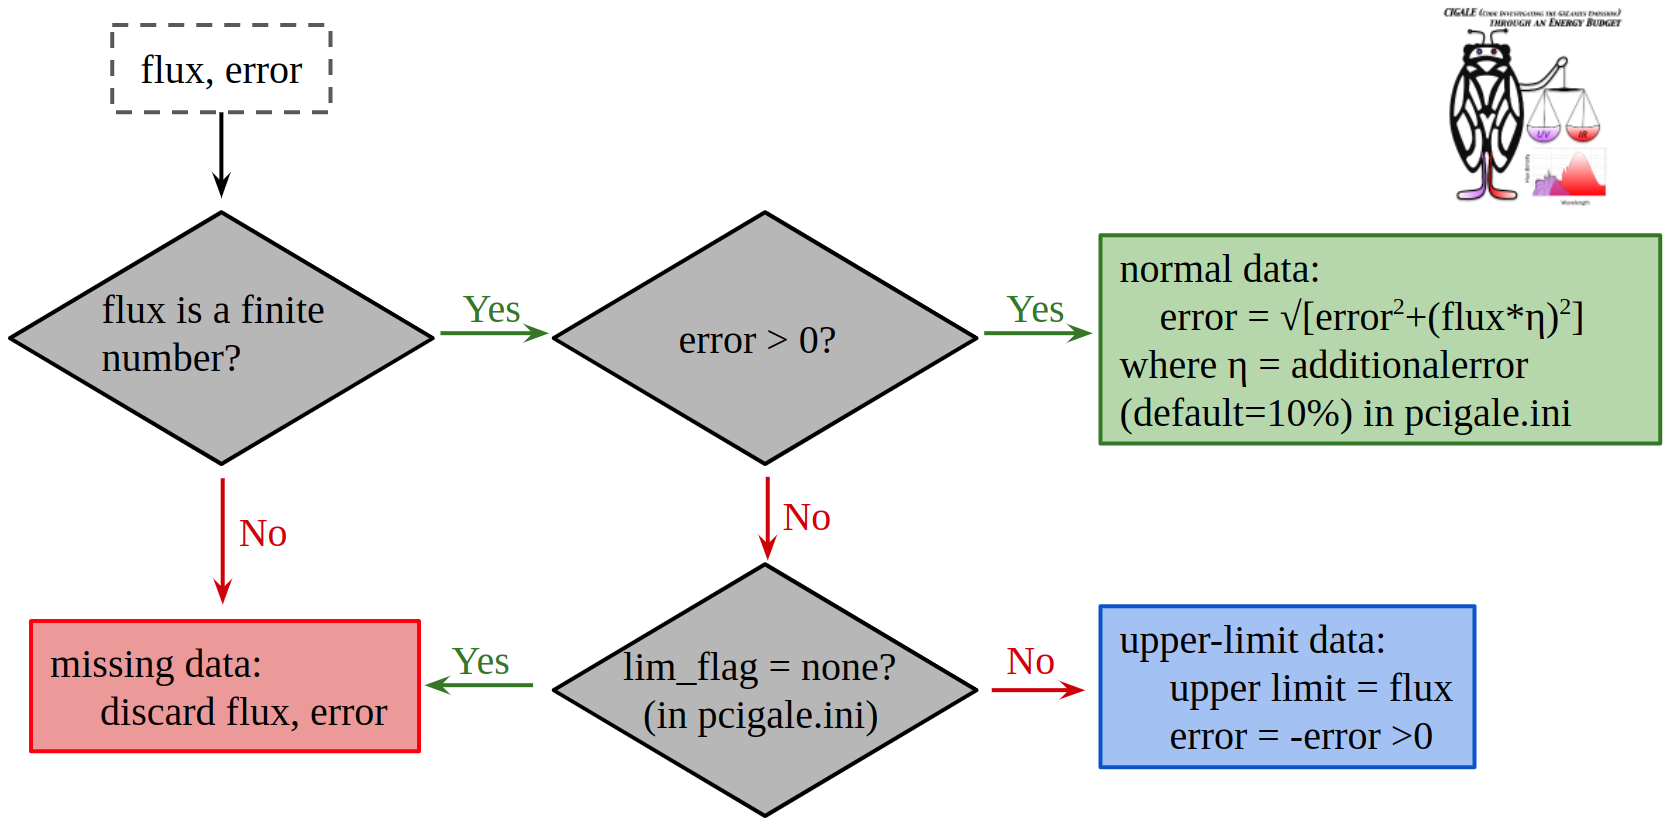
\includegraphics[width=\columnwidth]{pdfanalysis/flux_fluxerr.png}
\caption[How \xcig\ manages fluxes and flux errors]{This figure presents how \xcig\ manages (flux, error) for each filter.}
\label{fig:flux_fluxerr}
\end{figure}

\subsubsection{X-ray filters and fluxes}\label{sec:xray}
As explain in \cite{yang20}, \xcig\ requires that the input \xray\ fluxes are intrinsic.
This means that the energy-dependent instrumental response should have been corrected. 
Therefore, the \xray\ filters should be flat, i.e. boxcar-shaped. 
Fig.~\ref{fig:boxcar} presents an example \xray\ filter for 2--7~keV. 
\xcig\ includes a few filters for typical \xray\ bands. 
You can also create your own \xray\ filters. 
For your convenience, we provide a Python code (code/xray\_filter.py) to generate boxcar filters for a given \xray\ band. 
For example, you can run it as \\
\$ \textit{python} \\
$>>>$ \textit{import xray\_filter} \\
$>>>$ \textit{xray\_filter.write\_boxcar\_filter(``1to5.dat'', ``1to5'', 1, 5)} \\
will write a filter named ``1to5.dat'' for 1--5~keV. 

\begin{figure}[ht]
\centering
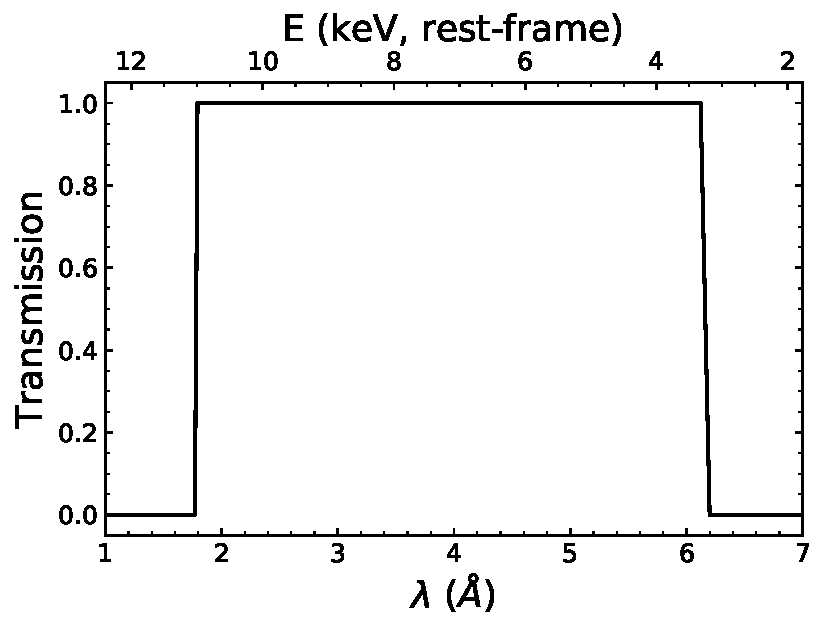
\includegraphics[width=0.6\columnwidth]{pdfanalysis/boxcar.pdf}
\caption[An example \xray\ boxcar filter for 2--7~keV]{An example \xray\ boxcar filter for 2--7~keV.}
\label{fig:boxcar}
\end{figure}

In \xray\ catalogs, the fluxes are often given in the cgs units of erg~s$^{-1}$~cm$^{-2}$. 
\xcig\ requires all inputs fluxes to be in units of mJy. 
Eq.~1 of \cite{yang20} gives the formula for the conversion. 
We also provide a Python code (``code/convert\_Fx.py'') to do this job. 
For example, \\
\$ \textit{python} \\
$>>>$ \textit{import convert\_Fx} \\
$>>>$ \textit{Fnu, Fnu\_err = convert\_Fx.convt\_Fx\_to\_Fnu([1e-16, 1e-15], [3e-17, 2e-16], 2, 7)} \\
will convert \hbox{2--7}~keV fluxes of [1e-16, 1e-15] erg~s$^{-1}$~cm$^{-2}$ and errors of [3e-17, 2e-16] erg~s$^{-1}$~cm$^{-2}$ to mJy fluxes (``Fnu'') and flux errors (``Fnu\_err''). 
These outputs of ``Fnu'' and ``Fnu\_err'' can then be written to \xcig\ input data.

\subsection{Configuration and Run}\label{sec:config}
Open terminal, cd to your working directory. \\
\$ \textit{pcigale init} \\
will initialize configuration files called ``pcigale.ini'' and ``pcigale.ini.spec''.
You only need to edit ``pcigale.ini''.
There are five parameters in this file (with many commentary words starting with \#): ``data\_file'', ``parameters\_file'', ``sed\_modules'', ``analysis\_method'', ``cores''. 
\begin{itemize}
    \item ``data\_file'' is the input data file (\S\ref{sec:data}). 
    \item ``parameters\_file'' is the optional file when simulating data (see \S\ref{sec:saveflux}). It should be  empty when fitting observed data. 
    \item ``sed\_modules'' lists the names of the SED modules that will be used in the run. 
    The available modules are listed in the commentary parts of the ``pcigale.ini'' file. 
    The module names should follow the order given in the commentary parts. 
    \item ``analysis\_method'' is \xcig\ mode. Should be ``pdf\_analysis'' for data-fitting purpose.
    \item ``cores'' is the number of CPU cores that will be used. Note that increasing the number of cores may not necessarily boost the speed. 
\end{itemize}
We provide two example runs of \hbox{AKARI-NEP} AGNs and SDSS QSOs \citep{yang20} along with this manual (``examples/akari\_nep\_xray\_agn'' and ``examples/sdss\_qso/''). 
In the test run, the configuration file reads:
\begin{itemize}
    \item[] \textit{data\_file = sdss\_qso.txt}
    \item[] \textit{parameters\_file = }
    \item[] \textit{sed\_modules = sfhdelayed, bc03, nebular, dustatt\_calzleit, dale2014, skirtor2016, xray, redshifting}
    \item[] \textit{analysis\_method = pdf\_analysis}
    \item[] \textit{cores = 4}
\end{itemize}
After setting the initial configuration file, run the following in terminal\\
\$ \textit{pcigale genconf} \\
which will generate the full configuration files ``pcigale.ini'' and ``pcigale.ini.spec''. 

Open ``pcigale.ini'', and you will find more parameters have been added. 
Following ``cores'', there are two parameters ``bands'' and ``properties''. 
You can see that \xcig\ already fills in the band and property names from the input data. 
But if you do not want to use some information, you can delete some entries.  

The other new parameters fall into two categorises, [sed\_modules\_params] and [analysis\_params]. 
[sed\_modules\_params] includes the configurations for each adopted SED module. 
These parameters should be self-explanatory, and we do not further explain them here. 
[sed\_modules\_params] determines the number of models that will be built. 
After finishing [sed\_modules\_params], you can check the number of models with \\
\$ \textit{pcigale check} \\
\textit{With this configuration cigale will compute 15966720 models.} \\

\noindent [analysis\_params] includes the configurations for the analysis, i.e.,
\begin{itemize}
    \item ``variables'' is the list of the physical properties to estimate in the Bayesian-like style. 
    The full list of properties can be found in Appendix~\hyperref[app:par]{A}.
    Note that this parameter only affects Bayesian results. 
    The best-fit (least-$\chi^2$) values for all properties are calculated in the results anyway.
    \item ``save\_best\_sed'' can be ``True'' or ``False''. 
    If ``True'', will save the best-fit SED and SFH models for each source. 
    \item ``save\_chi2'' can be ``none'', ``fluxes'', ``properties'', or ``all''. 
    If ``fluxes'', will save the raw $\chi^2$ for each photometric band for each source. 
    If ``properties'', will save $\chi^2$ for ``variables'' above for each source.
    If ``all'', will save $\chi^2$ for both photometric bands and ``variables''.
    If ``none'', will not save $\chi^2$.
    %The output files will be in {\sc numpy.memmap} format. 
    We provide a {\sc python} script ``code/read\_chi.py'' for reading the output $\chi^2$ file (in .npy format).
    \item ``lim\_flag'' can be ``none'' ``full'', or ``noscaling''. 
    If ``none'', will discard all upper limits in the input data (see Fig.~\ref{fig:flux_fluxerr}).
    If ``full'', will analyze upper limits using exact computation (slow speed). 
    If ``noscaling'' (default), will use an approximate method to deal with upper limits, which is a good balance between efficiency and reliability.
    \item ``mock\_flag'' can be ``True'' or ``False''.
    If ``True'', will create a mock catalog and analyze it. 
    This is a quick way to check if the physical properties can be constrained in a self-consistent way (see \S4.3 of \citealt{boquien19}).
    \item ``redshift\_decimals'' is the number of decimals to round the observed redshifts. 
    To disable rounding give a negative value.
    \item ``blocks'' is the number of blocks for the run.
    The default is 1, which is optimal for speed. 
    But if your computer memory is not enough, you can set it to $>1$. 
\end{itemize}
After completing ``pcigale.ini'', you can run \xcig\ with \\
\$ \textit{pcigale run} \\
Along with this manual, we provide an example configuration file, ``examples/sdss\_qso/pcigale.ini''.  

\subsection{Results}\label{sec:pdf_res}
After the run finishes, you can find the results in the ``out/'' directory. 
This directory contains:
\begin{itemize}
    \item ``results.txt'' (ASCII format) and ``results.fits'' (FITS format), the source-property catalog from the fitting.
    \item ``pcigale.ini'' and ``pcigale.ini.spec'', the used configuration files. 
    \item ``observations.txt'' and ``observations.fits'', the input observed data. 
    \item ``{SOURCE ID}\_best\_model.fits'' (exist if ``save\_best\_sed'' is set to ``True''), the best-fit SEDs for {SOURCE ID}, including the total and different components.
    \item ``{SOURCE ID}\_SFH.fits'' (exist if ``save\_best\_sed'' is set to ``True''), the best-fit SFH for {SOURCE ID}.
    \item ``{SOURCE ID}\_{PROPERTY}\_chi2-block-{BLOCK}.npy'' (exist if ``save\_chi2'' is set to ``True''), the raw $\chi^2$ of {PROPERTY} for {SOURCE ID} in {BLOCK}. 
    We provide a {\sc python} script to read these files (``code/read\_chi.py''). 
    \item ``mock\_observations.txt'', ``mock\_observations.fits'', ``results\_mock.txt'', and ``results\_mock.fits'' (exist if ``mock\_flag'' is set to ``True''), the mock catalog and fitting results. 
\end{itemize}
You can visualize the results with \textit{pcigale-plots} command. 
For example, \\
\$ \textit{pcigale-plots sed}\\
will generate the best-fit SED plot for each source in pdf format (``out/{SOURCE ID}\_best\_model.pdf'').
Fig.~\ref{fig:exm_sed} shows an example SED generated by the \textit{pcigale-plots} command.

\begin{figure}[ht]
\centering
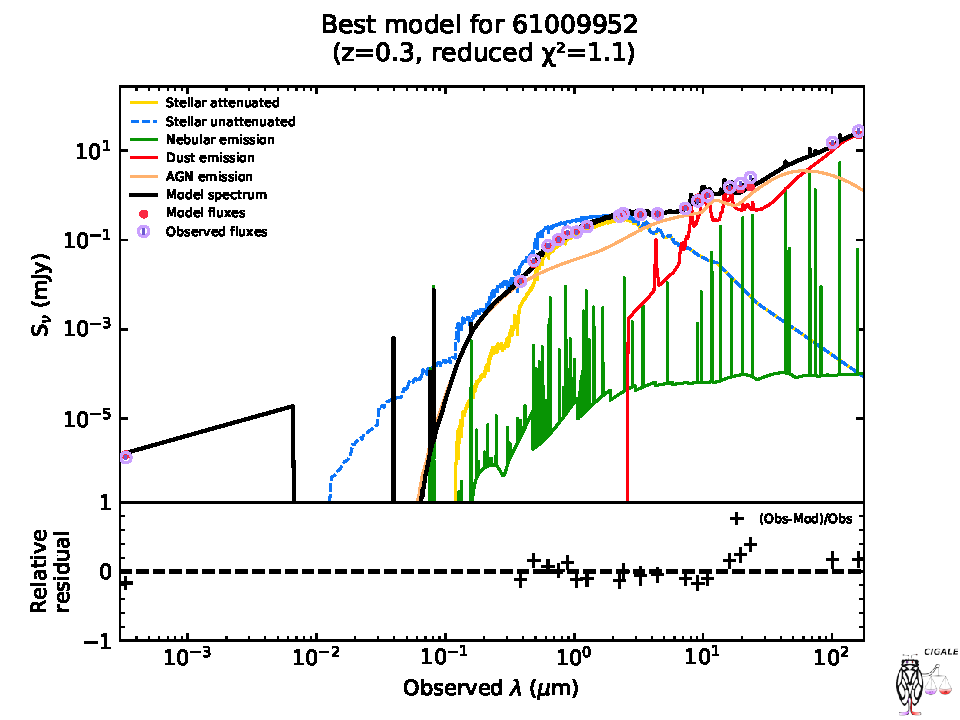
\includegraphics[width=\columnwidth]{pdfanalysis/exm_sed.pdf}
\caption[An example SED generated by the \textit{pcigale-plots} command]{An example SED generated by the \textit{pcigale-plots} command.}
\label{fig:exm_sed}
\end{figure}